\documentclass[prb,aps,twocolumn,showpacs,10pt]{revtex4-1}
\pdfoutput=1
\usepackage{dcolumn}% Align table columns on decimal point
\usepackage{bm}% bold math

%\usepackage{anysize}
\usepackage[colorlinks,hyperindex, urlcolor=blue, linkcolor=blue,citecolor=black, linkbordercolor={.7 .8 .8}]{hyperref}
\usepackage{graphicx}
%\usepackage{tabularx}
\usepackage{amsfonts}
\usepackage{amsmath}
\usepackage{amssymb}
\usepackage{amsbsy}
\usepackage{tikz}
%\usepackage{wrapfig}
%\usepackage{setspace}
%\usepackage{caption}
%\usepackage{fancyhdr}
\usepackage{nicefrac}
\usetikzlibrary{arrows,shapes,positioning}
\newenvironment{psmallmatrix}
  {\left[\begin{matrix}}
  {\end{matrix}\right]}
  
 \usepackage{listings}
\usepackage{color}

\definecolor{dkgreen}{rgb}{0,0.6,0}
\definecolor{gray}{rgb}{0.5,0.5,0.5}
\definecolor{mauve}{rgb}{0.58,0,0.82}

\lstset{frame=tb,
  language=Java,
  aboveskip=3mm,
  belowskip=3mm,
  showstringspaces=false,
  columns=flexible,
  basicstyle={\small\ttfamily},
  numbers=none,
  numberstyle=\tiny\color{gray},
  keywordstyle=\color{blue},
  commentstyle=\color{dkgreen},
  stringstyle=\color{mauve},
  breaklines=true,
  breakatwhitespace=true,
  tabsize=3
}


\newcommand{\etal}{{\it et~al.}}

\graphicspath{{benchmark/}}

\begin{document}

\title {Project 2}

\author{Jane Kim}
\affiliation{Physics 480: Computational Physics}
\date{\today}


\begin{abstract}

\vspace*{5mm}
\noindent In this project, we developed a code that implements Jacobi's rotation algorithm to solve for the eigenvalues and eigenvectors of a real, symmetric matrix. The algorithm was used to approximate the solutions to three differential equations for three physical situations. Mathematical properties of the algorithm were tested and the approximated eigenvalues were compared with the analytic forms and the eigenvalues calculated from Armadillo's functions. The algorithm passed all unit tests, but matrices with dimensions $\geq 400$ required over ten minutes of computation time.
\end{abstract}



\maketitle

\section{Introduction}

Many problems in physics are difficult, if not impossible, to solve analytically. However, in many cases, they can be reduced to relatively simple eigenvalue problems which can be solved numerically. In this project, we developed an eigenvalue and eigenvector solver using Jacobi's algorithm for real, symmetric matrices in order to solve three different examples of such problems with varying levels of complexity.
\subsection{Buckling Beam}
For the simplest of the three problems, we consider a beam of length $L$, whose vertical displacement in the $y$-direction is $u(x)$ for $x \in [0,L]$. If $R$ is some constant which reflects the properties, such as the rigidity, of the beam and a force $F$ is applied at $x=L$ towards the origin, the vertical displacement $u(x)$ satisfies the differential equation
\begin{equation}
R\frac{d^2 u(x)}{dx^2} = -Fu(x),
\end{equation}
with homogenous boundary conditions $u(0)=u(L)=0$. Since different combinations of the physical paramters $F, R$, and $L$ can yield the same solution, it is beneficial to introduce the dimensionless quantity $\rho = \frac{x}{L}$ to scale the differential equation. Then (1) becomes
\begin{equation}
\frac{d^2 u(\rho)}{d\rho^2} = -\lambda u(\rho),
\end{equation}
where $\lambda = FL^2/R$ and $\rho \in [0,1]$ \cite{notes}. For a given number of mesh points $N$, we can obtain a discretized approximation to $u(\rho)$ by rewriting (2) as an eigenvalue problem given by
\begin{align}
\label{eqn:eqlabel}
\begin{split}
A\vec{u} &= \lambda \vec{u},
\\
\begin{psmallmatrix} d&a& \\
a&d&a\\
&\ddots&\ddots&\ddots\\
&&a&d&a\\
&&&a&d\\
\end{psmallmatrix}
\begin{psmallmatrix}
u_1\\u_2\\ \vdots \\ u_{N-2}\\ u_{N-1}
\end{psmallmatrix}&=
\lambda
\begin{psmallmatrix}
u_1\\u_2\\ \vdots \\ u_{N-2}\\ u_{N-1}
\end{psmallmatrix},\\
u_i &= u(\rho_i),\\
\rho_i &= ih,\\
\end{split}
\end{align}
where $d = 2/h^2$, $a = -1/h^2$, and $h = 1/N$ is the step size. At the endpoints, $u_0 = u_N = 0$. This Toeplitz matrix has analytic eigenvalues
\begin{equation}
\lambda_i = d+2a\cos \left( \frac{i \pi}{N+1} \right) , \ \ \ i = 1, 2, ..., N-1,
\end{equation}
which we used to check the accuracy of the eigenvalue solver.

\subsection{One Electron Harmonic Oscillator}
Jacobi's algorithm is applicable for any real, symmetric matrix, so the same program we developed to solve the buckling beam problem can be used to solve the time-independent Schr{\"o}dinger equation for one and two electrons in a three-dimensional harmonic oscillator potential. For one electron with $\ell=0$, we substitute $R(r)=u(r)/r$ into the radial equation and introduce a dimensionless variable $\rho = r/\alpha$ to obtain
\begin{equation}
\left( -\frac{\hbar^2}{2m\alpha^2} \frac{d^2}{d\rho^2} + \frac{1}{2}m\omega^2\alpha^2\rho^2 \right) u(\rho) = E u(\rho). 
\end{equation}
By fixing $\alpha=(\hbar/m\omega)^{1/2}$ and letting $\lambda=2m\alpha^2 E/\hbar^2 = 2E/\hbar\omega$\cite{notes}, (5) becomes 
\begin{equation}
\left( -\frac{d^2}{d\rho^2} + \rho^2 \right) u(\rho) = \lambda u(\rho).
\end{equation}
The boundary conditions are $u(0)=\lim_{\rho \rightarrow \infty} u(\rho)=0$, but due to the finite nature of discretizing the differential equation, we must define a window $[\rho_{min}, \rho_{max}]$ on which to compute the eigenvalues and eigenvectors. Then the discretized equation is given by
\begin{equation}
-\frac{1}{h^2} u_{i-1} + \left( \frac{2}{h^2} + \rho_i^2 \right) u_i -\frac{1}{h^2} u_{i+1} = \lambda u_i, 
\end{equation}
where $h=(\rho_{max}-\rho_{min})/N$, $\rho_i = \rho_{min} + ih$, $i = 1, ..., N-1$. Therefore, the only difference between this eigenvalue problem and the buckling beam problem is that the diagonal elements have an additional non-constant term $\rho_i^2$. This problem also has analytic eigenvalues given by $\lambda = 3, 7, 11, 15, ...$.

\subsection{Two Electron Harmonic Oscillator}

When the repulsive Coulomb interaction is ignored, the Hamiltonian $H_0$ for two electrons in a harmonic oscillator can be written with respect to the center-of-mass coordinate $\mathbf{R}=(\mathbf{r}_1+\mathbf{r}_2)/2$ and the relative coordinate $\mathbf{r}=\mathbf{r}_1-\mathbf{r}_2$:
\begin{align}
\label{eqn:eqlabel}
\begin{split}
H_0(r,R) &= H_0(r) + H_0(R),\\
H_0(r) &=-\frac{\hbar^2}{m} \frac{d^2}{dr^2} + \frac{1}{4} k r^2,\\
H_0(R) &= -\frac{\hbar^2}{4m} \frac{d^2}{dR^2} + kR^2,
\end{split}
\end{align}
where $k=m\omega^2$. Then with the Coulomb interaction
\begin{equation}
V(r) = \frac{\beta e^2}{r}, \ \ \ \beta e^2 = 1.44 \ \text{eV} \cdot \text{nm},
\end{equation}
the $r$-dependent Schr{\"o}dinger equation is given by
\begin{equation}
H(r)\psi(r)=[H_0(r)+V(r)]\psi(r)=E_r \psi(r)
\end{equation}
As with one electron case, we substitute the dimensionless variable $\rho=r/\alpha$ in (10) to obtain
\begin{equation}
\left( -\frac{d^2}{d\rho^2} + \omega_r^2\rho^2 + \frac{1}{\rho}\right) \psi(\rho) = \lambda\psi(\rho).
\end{equation}
Here, we have fixed $\alpha=\hbar^2/m\beta e^2$ and defined $\lambda = $ 
$m\alpha^2E/\hbar^2$. Thus the two electron case simply adds another term $1/\rho_i$ to the diagonal elements of $A$ from the one electron case. 

\section{METHOD}

Jacobi's rotation algorithm is an iterative method for approximating the eigenvalues and eigenvectors of a real, symmetric, $N\times N$ matrix. Say we have such a matrix  $A$, and it has a non-zero element $a_{k\ell}$ for some $k, \ell = 1,2,...,N$ and $k\neq \ell$. Let $J(k,l,\theta)$ be a rotation matrix with the form
\begin{equation}
J(k,l,\theta) = \begin{psmallmatrix}
&1&\cdots &0 &\cdots &0 &\cdots &0\\
&\vdots& &\vdots & &\vdots & &\vdots\\
&0&\cdots &c &\cdots &s &\cdots &0\\
&\vdots& &\vdots & &\vdots & &\vdots\\
&0&\cdots &-s &\cdots &c &\cdots &0\\
&\vdots& &\vdots & &\vdots & &\vdots\\
&0&\cdots &0 &\cdots &0 &\cdots &1\\
\end{psmallmatrix},
\end{equation}
where $J_{kk}=J_{\ell\ell}=\cos\theta=c$ and $J_{k\ell}=-J_{\ell k}=\sin\theta=s$. This matrix is orthogonal, so for some arbitrary angle $\theta$, conjugation of $A$ by $J(k,\ell,\theta)$ is given by
\begin{equation}
A'=J(k,\ell,\theta)^T A J(k,\ell,\theta),
\end{equation}
where $A'$ has the entries 
\begin{align}
a_{kk}'&=c^2a_{kk}+s^2a_{\ell\ell}-2csa_{k\ell}\\
a_{\ell\ell}'&=s^2a_{kk}+c^2a_{\ell\ell}+2csa_{k\ell}\\
a_{ik}'&=a_{ki}'=ca_{ik}-sa_{i\ell}, \ \ \ i\neq k, i \neq \ell\\
a_{il}'&=a_{li}'=ca_{i\ell}+sa_{ik}, \ \ \ i\neq k, i \neq \ell\\
a_{k\ell}'&=a_{\ell k}'=(c^2-s^2)a_{k\ell}+sc(a_{kk}-a_{\ell\ell})
\end{align}
We can calculate the special angle $\theta$ for which the elements $a_{k\ell}'$ and $a_{\ell k}'$ become zero using equation (18). In this way, Jacobi's algorithm diagonalizes the matrix $A$ by repeatedly applying similarity transformations of the form (13) to "zero out" the off-diagonal elements $a_{k\ell}$. The largest off-diagonal element is chosen to increase efficiency. The eigenvalues of $A$ are the diagonal elements of the resulting matrix.\\

To calculate $\theta$, we set (18) equal to zero to yield
\begin{equation}
\frac{a_{\ell\ell}-a_{kk}}{a_{k\ell}} = \frac{c^2-s^2}{cs} = \frac{c}{s}-\frac{s}{c} = \frac{1}{t}-t,
\end{equation}
where $\tan\theta=t=s/c$. We define $\tau = (a_{\ell\ell}-a_{kk})/2a_{kl}$ so that (19) can be rewritten as the quadratic equation
\begin{equation}
t^2+2\tau t - 1 = 0,
\end{equation}
which has the analytic solutions $t=-\tau\pm \sqrt{1+\tau^2}$. Once $t$ is known, $c$ and $s$ are calculated using 
\begin{equation}
c = \frac{1}{\sqrt{1+t^2}}, \ \ \  s=tc.
\end{equation}
In addition, the products $c^2, s^2$, and $cs$ are precalculated before applying equations (14) and (15).\\

Suppose the matrix $A$ is (nearly) diagonal after $n$ rotations, i.e. 
\begin{equation}
D=J_n^T \cdots J_2^T J_1^T A J_1 J_2 \cdots J_n
\end{equation}
for some rotation matrices $J_i$ and diagonal matrix $D$. Then the eigenvectors are simply given by the columns of the product $J_1J_2\cdots J_n$.

\section{Implementation}

\subsection{Jacobi's Algorithm}

The bulk of Jacobi's algorithm can be broken down into two parts: the search for the largest off-diagonal element $a_{k\ell}$, called a pivot, followed by the corresponding rotation of the form (13). Accordingly, we developed a function called \texttt{get\_pivot} which stores the indices $k,\ell$ of the largest element of $A$ above the diagonal (since $A$ is symmetric).

\begin{lstlisting}
// jacobi.cpp
void get_pivot(mat& A, int N, int& k, int& l){
	double Aij,max_offdiag = 0.0;
	for(int i = 0; i < N-1; i++){
		for(int j = i+1; j < N; j++){
			Aij = fabs(A(i,j));
			if(Aij > max_offdiag){
				max_offdiag = Aij;
				k = i;
				l = j;
			}
		}
	}
}
\end{lstlisting}

\noindent Meanwhile, another function called \texttt{rotate} carries out the transformation $A'=J(k,\ell,\theta)^TAJ(k,\ell,\theta)$ and right-multiplies a matrix $V$ by $J(k,\ell,\theta)$. $V$ is initialized as the identity matrix before the first rotation so that the columns of the resulting matrix are the eigenvectors of $A$. 

\begin{lstlisting}
// jacobi.cpp
void rotate(mat& A, mat& V, int k, int l, int N){

	// zero out A(k,l)=A(l,k)
	if( A(k,l) != 0.0 ){

		double c, s, t, tau;
		double cc, ss, cs;
		double Aik, Ail, Vik, Vil;
		double Akk = A(k,k), All = A(l,l), Akl = A(k,l);

		// calculate angle of rotation
		tau = 0.5*(All-Akk)/Akl;
		if(tau >= 0.0){ t = -tau+sqrt(1.0+tau*tau); }
		else{ t = -tau-sqrt(1.0+tau*tau); }

		cc = 1.0/(1.0+t*t);
		ss = 1.0-cc;
		cs = t*cc;
		c = sqrt(cc);
		s = t*c;

		// perform rotation
		A(k,l) = 0.0;
		A(l,k) = 0.0;
		A(k,k) = cc*Akk+ss*All-2.0*cs*Akl;
		A(l,l) = ss*Akk+cc*All+2.0*cs*Akl;
		for(int i = 0; i < N; i++){

			if( (i!=k) && (i!=l) ){
				Aik = A(i,k);
				Ail = A(i,l);
				A(i,k) = c*Aik-s*Ail;
				A(i,l) = c*Ail+s*Aik;
				A(k,i) = A(i,k);
				A(l,i) = A(i,l);
			}

			// rotate eigenvectors 
			Vik = V(i,k);
			Vil = V(i,l);
			V(i,k) = c*Vik-s*Vil;
			V(i,l) = s*Vik+c*Vil;
		}
	}

	else{ cout << "ERROR: These elements are already zero!" << endl; } 
}
\end{lstlisting}

\noindent $A$ is considered diagonalized after applying \texttt{get\_pivot} and \texttt{rotate} until the sum of squares of the off-diagonal elements is smaller than some fixed number $\epsilon$. This sum is calculated by a function called \texttt{offdiag\_sq}, which uses fact that $A$ is symmetric to reduce the number of floating point operations by a factor of two. Finally, for ease and readability, Jacobi's algorithm is implemented by repeatedly calling these three functions using \texttt{jacobi}:

\begin{lstlisting}
// jacobi.cpp 
void jacobi(mat& A, mat& V, int N){

	double epsilon = 1E-8;
	int k, l;

	while(offdiag_sq(A,N) > epsilon){
		get_pivot(A, N, k, l);
		rotate(A, V, k, l, N);
	}
}
\end{lstlisting}

To use \texttt{jacobi}, a matrix $A$ must first be initialized as the matrix we wish to diagonalize, and a matrix $V$ is initialized as the identity matrix.


\subsection{Unit Tests}

There are several tests we can use to check that the program we developed performs as expected. For example, similarity transformations with orthogonal matrices preserve the Frobenius norm of the matrix $A$, i.e.
\begin{equation}
||A||_F = \sqrt{\sum_{i=1}^N \sum_{i=1}^N a_{ij}}
\end{equation}
is preserved under (13). A function \texttt{norm\_sq} calculates the square of the Frobenius norm by adding the square of the diagonal elements to \texttt{offdiag\_sq}. Since Jacobi's algorithm is applicable to any real, symmetric matrix, $A$ and $V$ were initialized as the following:
\begin{lstlisting}
mat R = randu<mat>(N,N);
mat A = R.t()*R;
mat U = eye<mat>(N,N);
\end{lstlisting}
Then the test requires that \texttt{norm\_sq} has the same value before and after implementing the rotation algorithm.\\

Another simple test involves checking that the function \texttt{get\_pivot} correctly identifies the indices of the largest off-diagonal element. This is simple to execute, since $A$ can be any matrix whose largest element is known. In our case, $A$ was defined so that the largest element was the last element of the superdiagonal.\\

Since $V$ is actually the product of orthogonal matrices, the columns of $V$ (i.e. the eigenvectors of $A$) should be orthogonal. To perform this test, $A$ was initialized as a random, real, symmetric matrix. Then after implementing the rotation algorithm, the dot products of every pair of eigenvectors were calculated and required to be zero. \\

The eigenvalues of $A$ resulting from diagonalization can be checked in a few ways. For instance, if $A$ is a tridiagonal Toeplitz matrix given by (3), the analytic eigenvalues are given by (4). This test is straightforward to write, but it should be noted that the eigenvalues of $A$ after diagonalization are not given in ascending order, so they must be sorted before comparing to (4). For a general real, symmetric matrix, the eigenvalues can be compared to the eigenvalues obtained by Armadillo. 


\section{Results}

\subsection{Buckling Beam}

For the buckling beam problem, the eigenvalues of a tridiagonal Toeplitz matrix were calculated using Jacobi's rotation algorithm. Since such a matrix has analytic eigenvalues for all $N$ according to equation (14), the calculated eigenvalues closely resembled the analytic values for $N\leq 400$ (at least eight leading digits after the decimal point). Calculations for $N>400$ required well over 10 minutes of computation time, so they will not be discussed here. 
\begin{center}
\begin{tabular}{|c|c|c|c|}
\hline
$N$ & $n$ & time (s) & $n/N^2$ \\
\hline
\hline
50 & 3877 & 0.189517  &1.551\\
\hline
100 & 15940 & 2.2092& 1.594\\
\hline
150 & 36361 & 13.2449&1.616\\
\hline
200 & 65318 & 34.9609&1.633\\
\hline
250 & 102591 & 101.189&1.641\\
\hline
300 & 147616 & 183.099&1.640\\
\hline
350 & 203076 & 365.616 & 1.648\\
\hline
400 & 266663 & 635.14& 1.667\\
\hline
\end{tabular}

\vspace*{3mm}
\textit{Table 1.} The number of transformations (n) and the computation time required to diagonalize a tridiagonal Toeplitz matrix of dimension $N$.
\end{center}

From the table above, it is clear to see that the number of iterations $n$ is approximately proportional to $N^2$, with a proportionality constant somewhere between $3/2$ and $5/3$ for $N \leq 400$. The proportionality constant steadily increases as $N$ increases.

\subsection{One Electron Harmonic Oscillator}

Jacobi's algorithm was used to determine the energies and the corresponding wavefunctions for a single electron in a harmonic oscillator potential. The modified wavefunctions $u(\rho)$ for the first three energies are plotted in Figure 1. This problem has analytic eigenvalues as well, but unlike the buckling beam problem, the calculated eigenvalues approach the analytic values as the step size $h$ becomes small. If we fix $\rho_{min}$ at zero, there are two parameters which determine the size of $h$: $\rho_{max}$ and $N$. The following tables contain the calculated eigenvalues for various combinations of $\rho_{max}$ and $N$. 

\begin{center}
$\rho_{max} = 5$\\
\begin{tabular}{|c|c|c|c|c|}
\hline
exact & $N=50$ & $N=150$& $N=250$& $N=350$\\
\hline
\hline
3 & 2.99699&2.99966 & 2.99988 & 2.99994\\
\hline
7 & 6.98495 & 6.99829 & 6.99938 & 6.99969\\
\hline
11 & 10.9634 & 10.996 & 10.9987 & 10.9994\\
\hline
15 & 14.9374&14.9981 & 15.003 & 15.0044\\
\hline
19 & 18.959 & 19.0602 & 19.0685 & 19.0707\\
\hline
23 & 23.2355 & 23.4045 & 23.4184 & 23.4222\\
\hline
\end{tabular}
\vspace*{3mm}

$\rho_{max} = 10$\\
\begin{tabular}{|c|c|c|c|c|}
\hline
exact & $N=50$ & $N=150$& $N=250$& $N=350$\\
\hline
\hline
3 & 2.98793&2.99863 & 2.9995 & 2.99975\\
\hline
7 & 6.93939 & 6.99314 & 6.99752 & 6.99873\\
\hline
11 & 10.8514 & 10.9833 & 10.9939 & 10.9969\\
\hline
15 & 14.7233 &14.969 & 14.9888 & 14.9943\\
\hline
19 & 18.5545 & 18.9503 & 18.982 & 18.9908\\
\hline
23 & 23.3442 & 22.9271 & 22.9737 & 22.9865\\
\hline
\end{tabular}
\vspace*{3mm}

\textit{Table 2.} The first six eigenvalues for $\rho_{max} = 5$ (top) and $\rho_{max} = 10$ (bottom).
\vspace*{2mm}
\end{center}

Notice that for $\rho_{max}=5$, the first three eigenvalues approach the analytic values as $N$ increases. However, for the next three eigenvalues, the error appears to increase as $N$ becomes large. Doubling $\rho_{max}$ results in slightly less accurate approximations of the first four eigenvalues, but much more stable approximations of the next two eigenvalues as $N$ becomes large.
\begin{center}
\begin{figure*}
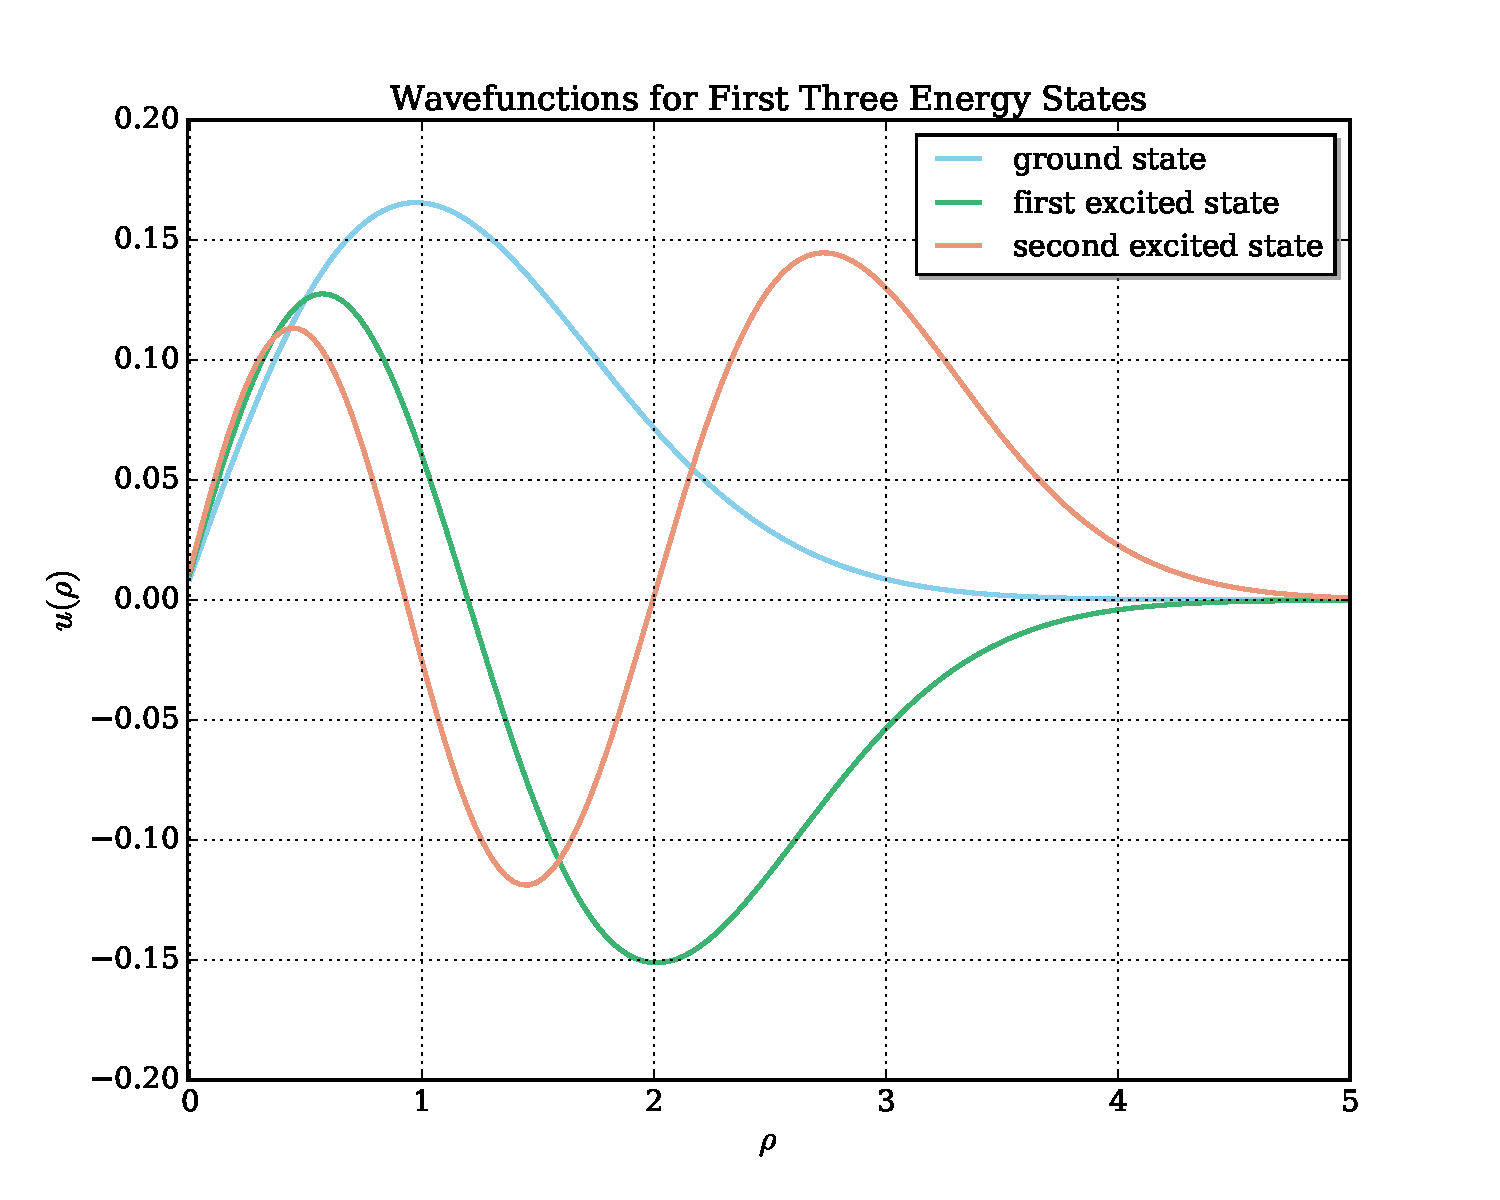
\includegraphics[scale=0.6]{wvfunc_1e.pdf}

\textit{Figure 1.} The approximate wavefunctions of the lowest three energy states for one electron in a three-dimensional harmonic oscillator potential are plotted above. Here, $\rho$ is the dimensionless variable defined in Section I. B and $N=400$.
\end{figure*}
\end{center}
To make sense of this behavior, we need to consider the problem we are trying to solve. In this instance, the eigenvalues correspond to energy states of the system, and in general, the wavefunctions corresponding to higher energy states extend to larger $\rho$ (Figure 1). Thus to obtain an accurate estimation of the $n^{th}$ eigenvalue we must first ensure that the window $\left[ \rho_{min},\rho_{max} \right]$ contains the region in which the $n^{th}$ wavefunction is non-zero. 

\subsection{Two Electron Harmonic Oscillator}

In this problem, the variable $\rho$ is a measure of the distance between the two electrons. The ground state probability densities for various harmonic oscillator frequencies $\omega_r$ are plotted in Figure 2. For narrow harmonic oscillator potentials, the Coulomb interaction appears to only alter the average distance between the electrons slighty. The Coulomb interaction has a much larger effect for wider potentials. This agrees with our expectations, since the Coulomb interaction is long-ranged and dominates the Hamiltonian when the harmonic oscillator potential is weak.


\begin{center}
\begin{figure*}
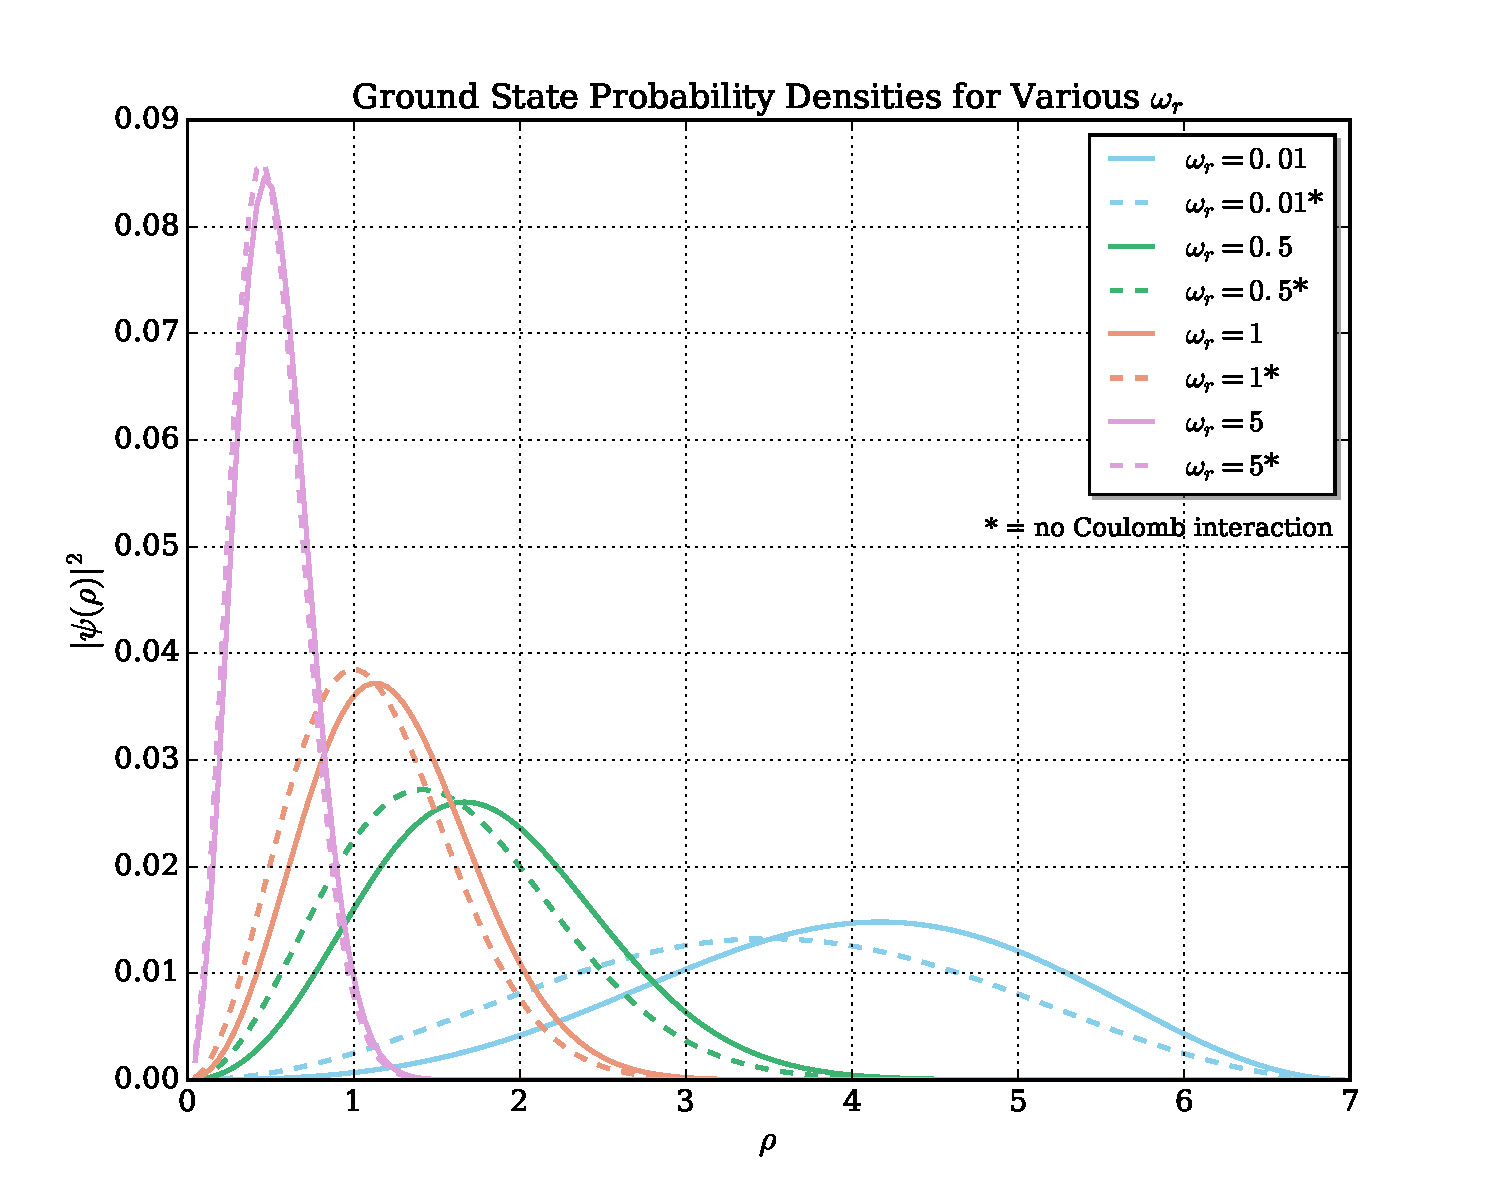
\includegraphics[scale=0.7]{prob_dens_2e.pdf}

\textit{Figure 2.} The approximate ground state probability densities for various $\omega_r$, with and without the Coulomb interaction. 
\end{figure*}
\end{center}

\section{Conclusion}

Jacobi's algorithm is a fairly straightforward method to calculate the eigenvalues and eigenvectors of a real, symmetric matrix. It can be applied to approximate the solutions of some differential equations, as we have discussed in this paper. However, it has its share of shortcomings. Most notably, the computation time required makes obtaining an accurate solution quite difficult for problems such as the one and two electron harmonic oscillator. As higher energies (or larger eigenvalues) are probed, $\rho_{max}$ must be extended accordingly to capture the non-zero activity of the corresponding wavefunctions. But then $N$ must also be increased to maintain a small mesh size.\\

The inefficiency of Jacobi's algorithm can be attributed to the fact that each rotation only "zeroes out" two off-diagonal elements, while altering two rows and two columns. It is possible that some rotations make zero elements become non-zero, thus requiring more iterations in the end.\\

Other algorithms should be considered to solve the three specific problems studied in this report. All of the matrices we encountered were not just symmetric, but also tridiagonal. Developing an algorithm with this specific form in mind can shorten the computation time significantly. \\






\newpage 
\begin{references}
\bibitem{notes} M. Hjorth-Jensen. "Computation Physics, Lecture Notes Fall 2015". University of Oslo. August 2015.
\end{references}

\end{document}
